 
\vspace{-4mm}\begin{center}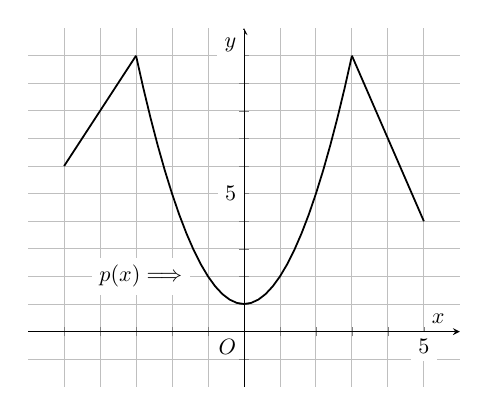
\begin{tikzpicture}[scale=0.8]
\begin{axis}[xmin=-6, xmax=6, ymin=-2, ymax=11,axis lines=center, grid=both, xtick={-5,-4,...,5}, ytick={-1, 0, ..., 10},xticklabel=\empty, yticklabel=\empty,]
\draw(axis cs: 0,0)node[anchor=north east]{$O$};
\draw(axis cs:5,0) node[rectangle,fill=white,anchor=north]{$5$};
\draw(axis cs:0,5) node[rectangle,fill=white,anchor=east]{$5$};
\draw(axis cs:0,10.4) node[rectangle, fill=white, anchor=east]{$y$};
\draw(axis cs:5.4,0) node[anchor=south, fill=white, anchor=south]{$x$};
\addplot[domain=-3:3,samples=31,thick,]{x^2+1};
\addplot[domain=3:5,samples=5,thick,]{-3*x+19};
\addplot[domain=-5:-3,samples=5,thick,]{2*(x+8)};
\draw(axis cs:-1.5,2)node[rectangle, fill=white, anchor=east]{$p(x)\Longrightarrow$};
\end{axis}
\end{tikzpicture}\end{center}
The complete graph of the function $p$ is shown in the $xy$-plane above.  Which of the following are equal to $5$?
\begin{enumerate}[label=\Roman*., ]
\item $p(-2)$
\item $p(2)$
\item $p(4)$
\end{enumerate}


\ifsat
	\begin{enumerate}[label=\Alph*)]
		\item I only. 
		\item II only. 
		\item III only. 
		\item I and II only. % 
	\end{enumerate}
\else
\fi

\ifacteven
	\begin{enumerate}[label=\textbf{\Alph*.},itemsep=\fill,align=left]
		\setcounter{enumii}{5}
		\item I only. 
		\item II only. 
		\item III only. 
		\addtocounter{enumii}{1}
		\item I and II only. % 
		\item None of these. 
	\end{enumerate}
\else
\fi

\ifactodd
	\begin{enumerate}[label=\textbf{\Alph*.},itemsep=\fill,align=left]
		\item I only. 
		\item II only. 
		\item III only. 
		\item I and II only. % 
		\item None of these. 
	\end{enumerate}
\else
\fi

\ifgridin
 I and II only. % 

\else
\fi

